\begin{activity}\label{A:0.2.1}
    Consider the exponential functions plotted in Figure \ref{F:0.2.Act1}
    \ba
        \item Which of the functions have common ratio $r > 1$?
        \item Which of the functions have common ratio $0<r< 1$?
        \item Rank each of the functions in order from largest to smallest $r$ value.
    \ea
    \begin{figure}[h!]
        \begin{center}
            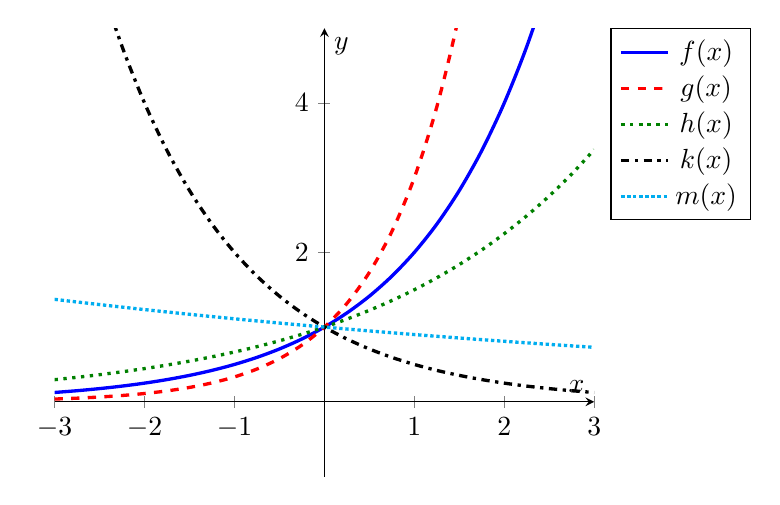
\begin{tikzpicture}
                \begin{axis}[axis lines=center, xlabel={$x$}, ylabel={$y$}, xmin=-3, xmax=3,
                    ymin=-1, ymax=5, domain=-3:3,legend pos=outer north east]
                    \addplot[smooth, blue, very thick] {2^x};
                    \addlegendentry{$f(x)$};
                    \addplot[smooth, red, very thick, dashed] {3^x};
                    \addlegendentry{$g(x)$};
                    \addplot[smooth, green!50!black, very thick, dotted] {1.5^x};
                    \addlegendentry{$h(x)$};
                    \addplot[smooth, black, very thick, dashdotted] {(0.5)^x};
                    \addlegendentry{$k(x)$};
                    \addplot[smooth, cyan, very thick, densely dotted] {(0.9)^x};
                    \addlegendentry{$m(x)$};
                \end{axis}
            \end{tikzpicture}
        \end{center}
        \caption{Exponential growth and decay functions} \label{F:0.2.Act1}
    \end{figure}
\end{activity}\aftera
